%--------- This is TPCN on h-BN/Cu-foil !
The Cu(111) support for the h-BN growth is reaplaced by a polycrystalline copper foil. The goal is to achieve the same ordering of molecules on the h-BN surface. The h-BN layer has been prepared by a dose of \SI{5E-7}{\milli\bar} borazine for 20min (4500\,L). During dosage the foil has been kept at \SI{820}{\degreeCelsius}.

When a h-BN spacer layer is introduced, the molecules decouple from the substrate, lowering their interaction with the afore-mentioned. This can be seen in a change of the molecules' footprint (rectangular $\rightarrow$ square).

They do not form ordered networks (like chains or squares) and lie rather loosely on the h-BN layer (compare 150807.142226.dat). They can easily be moved with the STM tip (1V, 10nA). In some areas, denser TPCN islands form. Here they lie right next to each other, each slightly shifted to match the neighbouring molecules and to achieve the dense packed regions. The same motiv was already investigated in the same system \cite{urgel_controlling_2015}.

During scanning (I=\SI{0.1}{\nA}, \SI{0.9}{\V} <U<\SI{1.3}{\V} ) of a group of molecules, a single molecules could be pushed out of the group (compare figure \ref{fig:TPCN-manipulation}. While the chain initially consisted of 3 molecules in a row, after scanning one of the molecular units moved to the left while the remaining two stay at their positions. A closer look to the moved molecule's geometry reveals deformation of the legs.

It was shown that the imminic nitrogen species within a 2H-TPP molecule strongly interact a Cu(111) surface, thus orient along high symmetry directions. .\cite{haq_clean_2011, buchner_diffusion_2011, gonzalez-moreno_following_2011, diller_self-metalation_2012, ditze_activation_2012,rojas_self-assembly_2010} Rotation and diffusion are limited.
\begin{figure}[!h]
%Gemessen im Oktober (um den 10ten) ... $$$
 \centering
 \subfigure[Image 1]{
 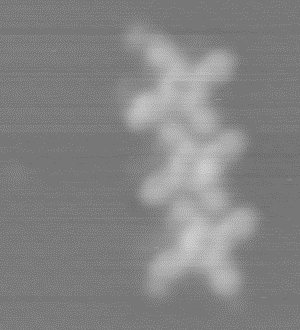
\includegraphics[width=0.3\textwidth]{./images/manipulation-2}
 }
 \subfigure[Image 2]{
 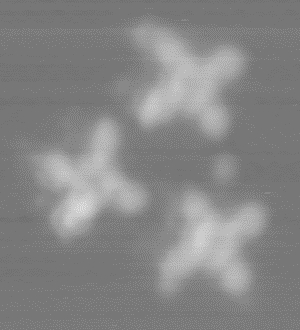
\includegraphics[width=0.3\textwidth]{./images/manipulation-1}
 }
 \subfigure[Overlay]{
 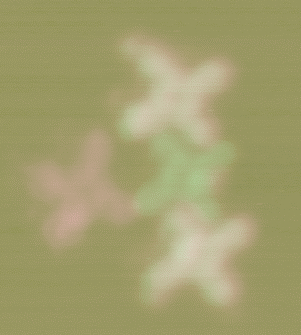
\includegraphics[width=0.3\textwidth]{./images/TPCN-manipulation}
 }
 \caption{Position change of TPCN group members. Central molecule is manipulated, color indicates its initial (a, green hue in c ) and final (b, red hue in c) position. Image (c) is created via an overlay of two sequential images. The upper and lower molecules do not shift thus sharing the same color.}
 \label{fig:TPCN-manipulation}
\end{figure}

\newpage
\begin{figure}[!h]
 \centering
 \subfigure[Loosely orderd molecules on the h-BN/Cu-foil surface.]{
  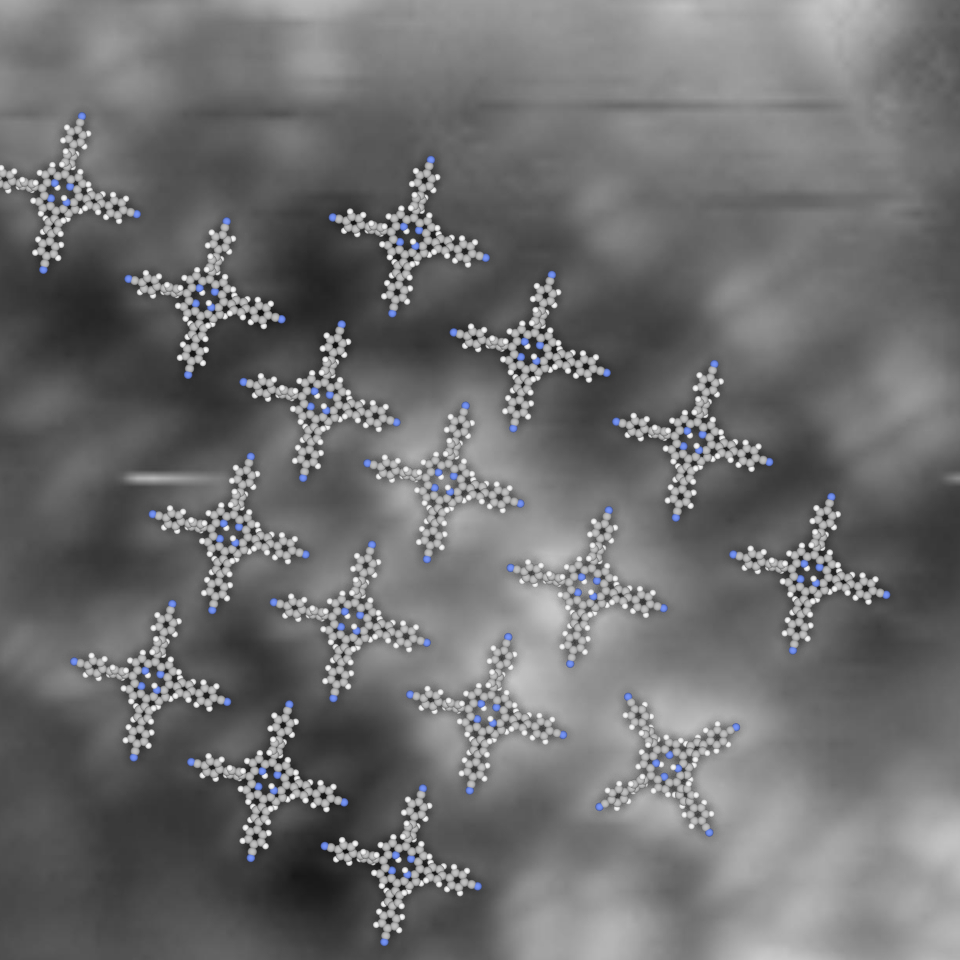
\includegraphics[width=0.45\textwidth]{./images/F150807-160006.jpg}
 }
 \subfigure[ Molecules do not always show ordering but in dense areas they do.]{
  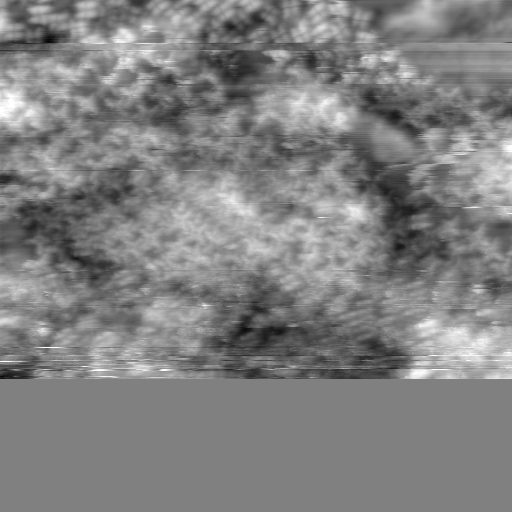
\includegraphics[width=0.45\textwidth]{./images/F150807-142226.jpg}
 }
\caption{There they form a motiv like in figure \ref{fig:TPCN-manipulation}a).}
\end{figure}

TPCN without added cobald form similar pattern on the h-BN/Cu-foil system (compare fig. 2b in \cite{urgel_controlling_2015}). Although the ordered areas were quiete rare, an ordered region has been found. Here the molecules are not strictly equi-distant or -rotated which makes it difficult to give an accurate unit cell for this type of motiv.
%--------- Describe how the TPCN form that network on h-BN --------- 

\newpage
\paragraph{Adding Co}
Introducing some cobald (15min, \SI{90}{\celsius}) in the system, this self-assembly changes. The molecules now form a 2D network, too, but are further apart. Their only connection point to the other molecules is the tip of their legs pointing to the adjacent leg of the neighboring molecule.

\begin{figure}[!h]
 \centering
  \subfigure[Zoomed view ($\SI{10}\times\SI{10}{\square\nm}$)]{
  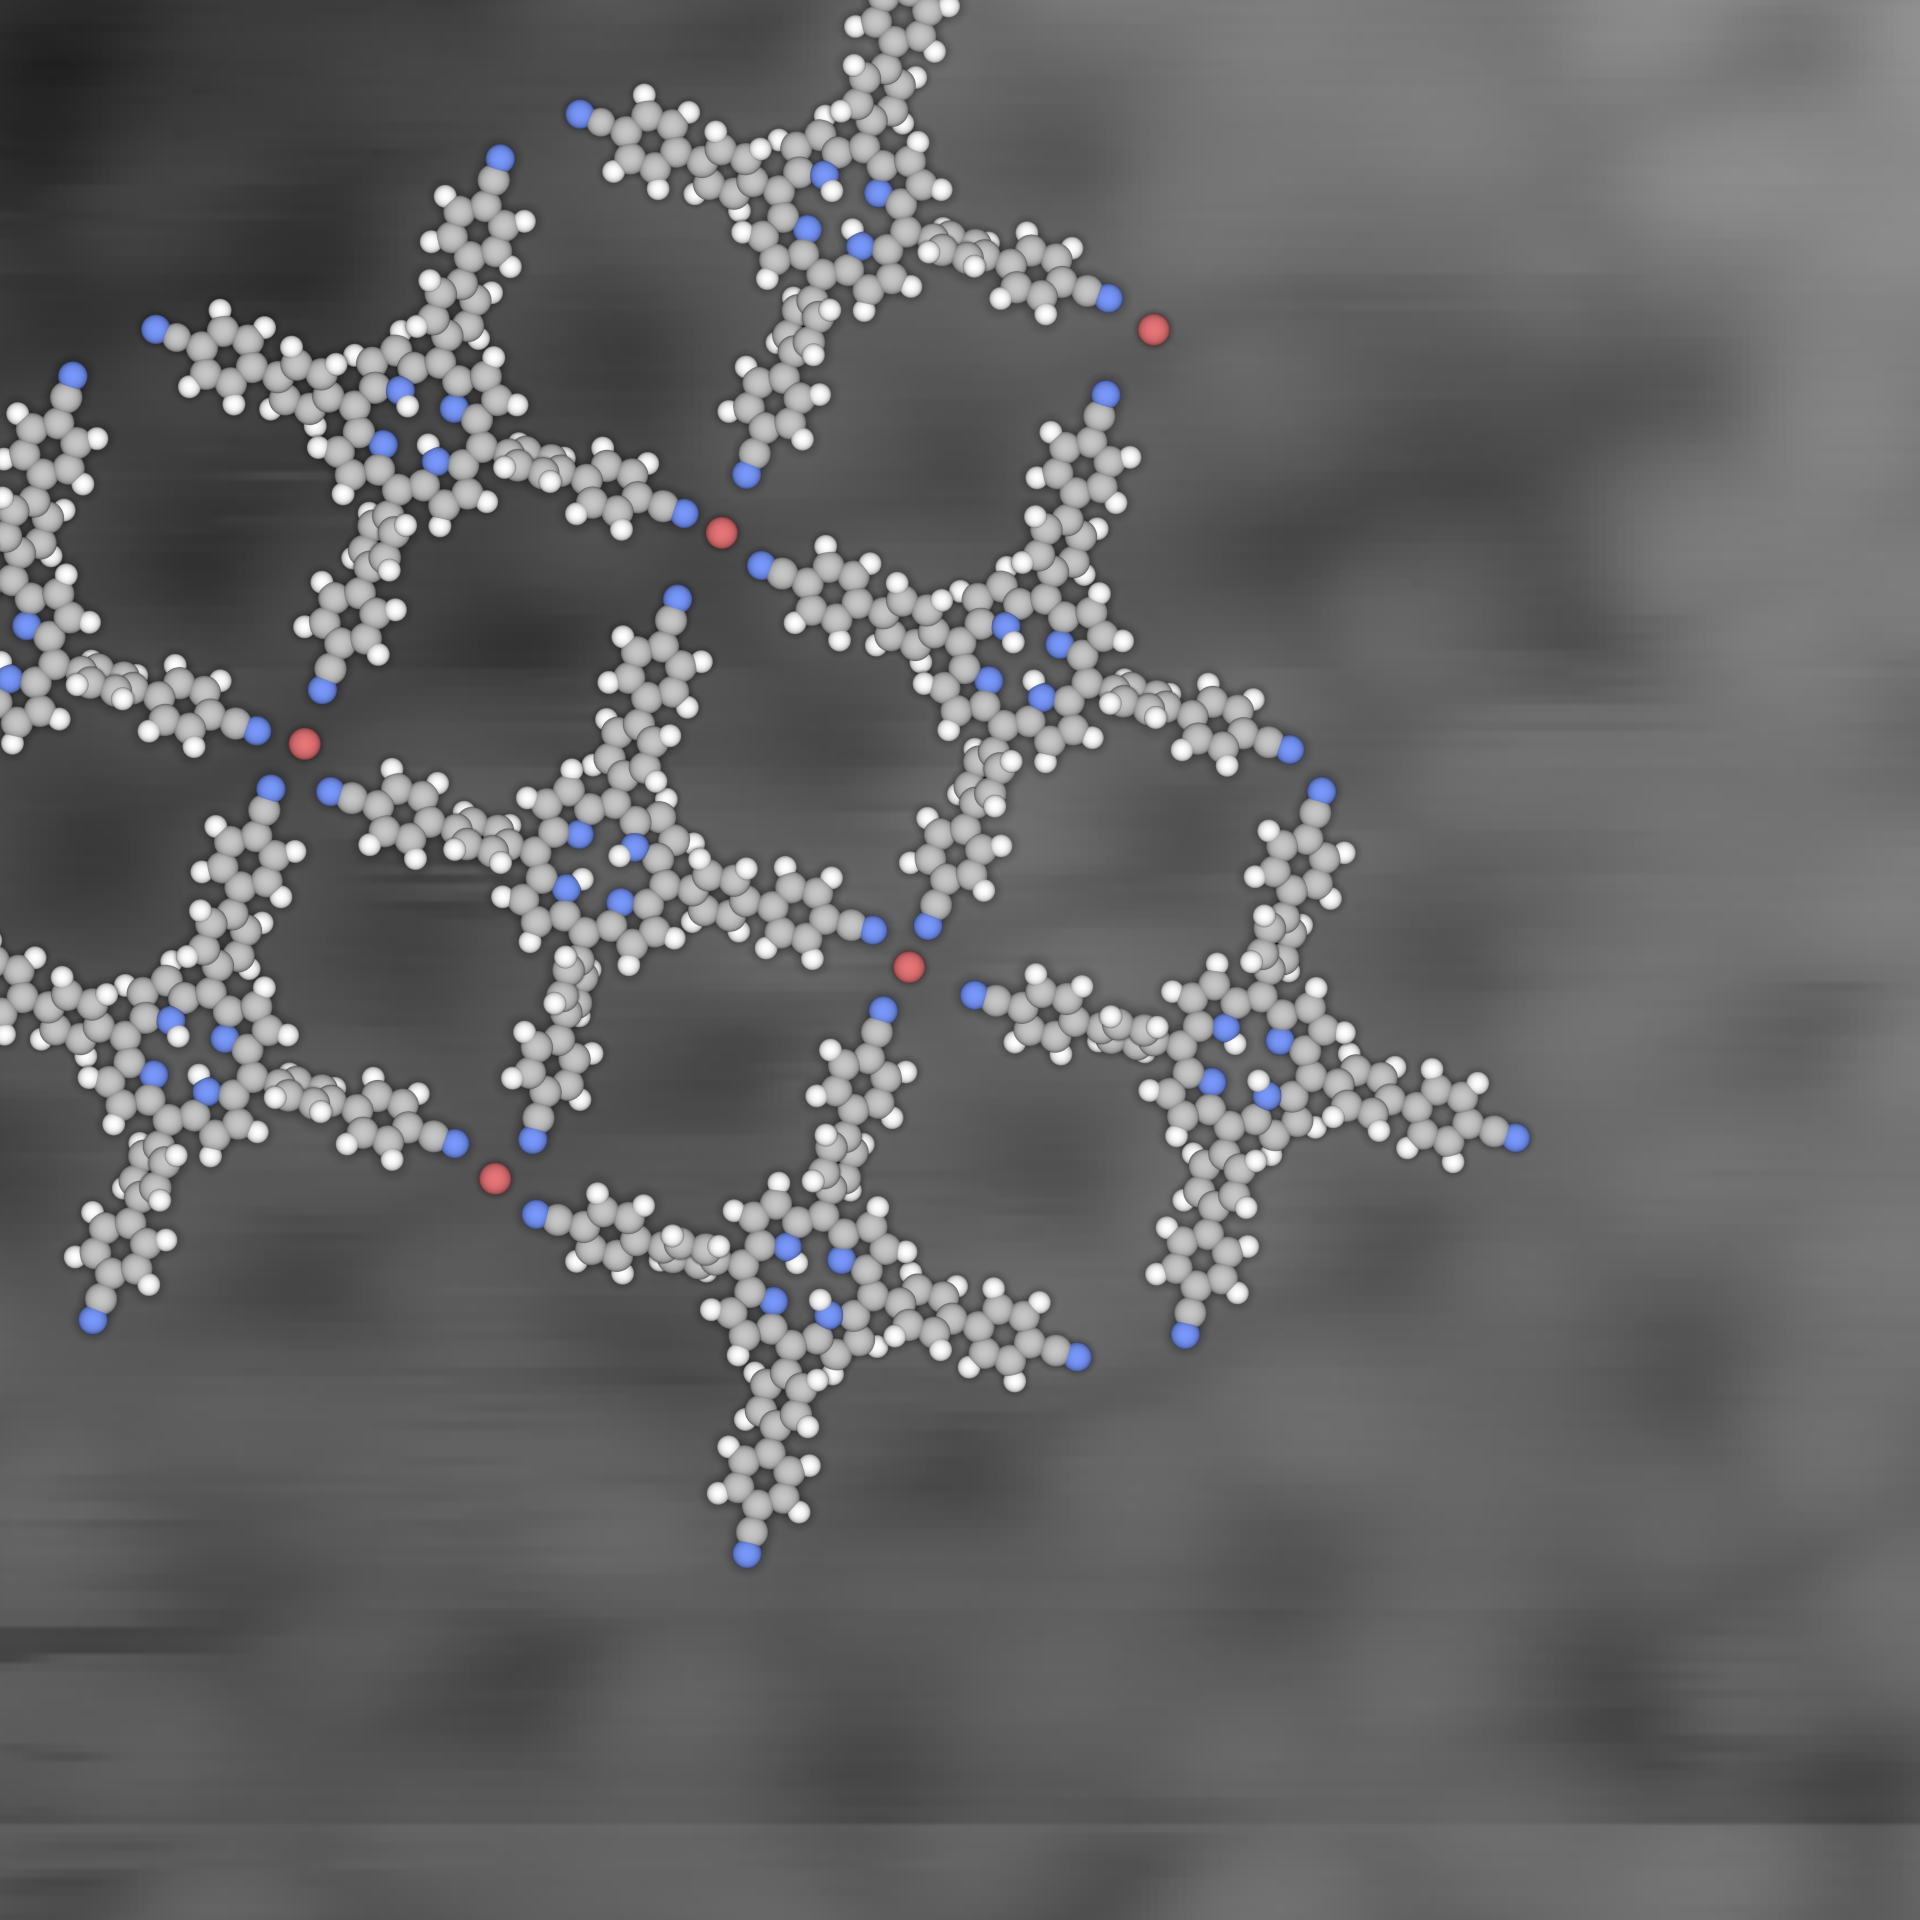
\includegraphics[width=0.45\textwidth]{./images/F150814-090450_01.jpg}
  }
  \subfigure[Zoomed view ($\SI{20}\times\SI{35}{\square\nm}$)]{
  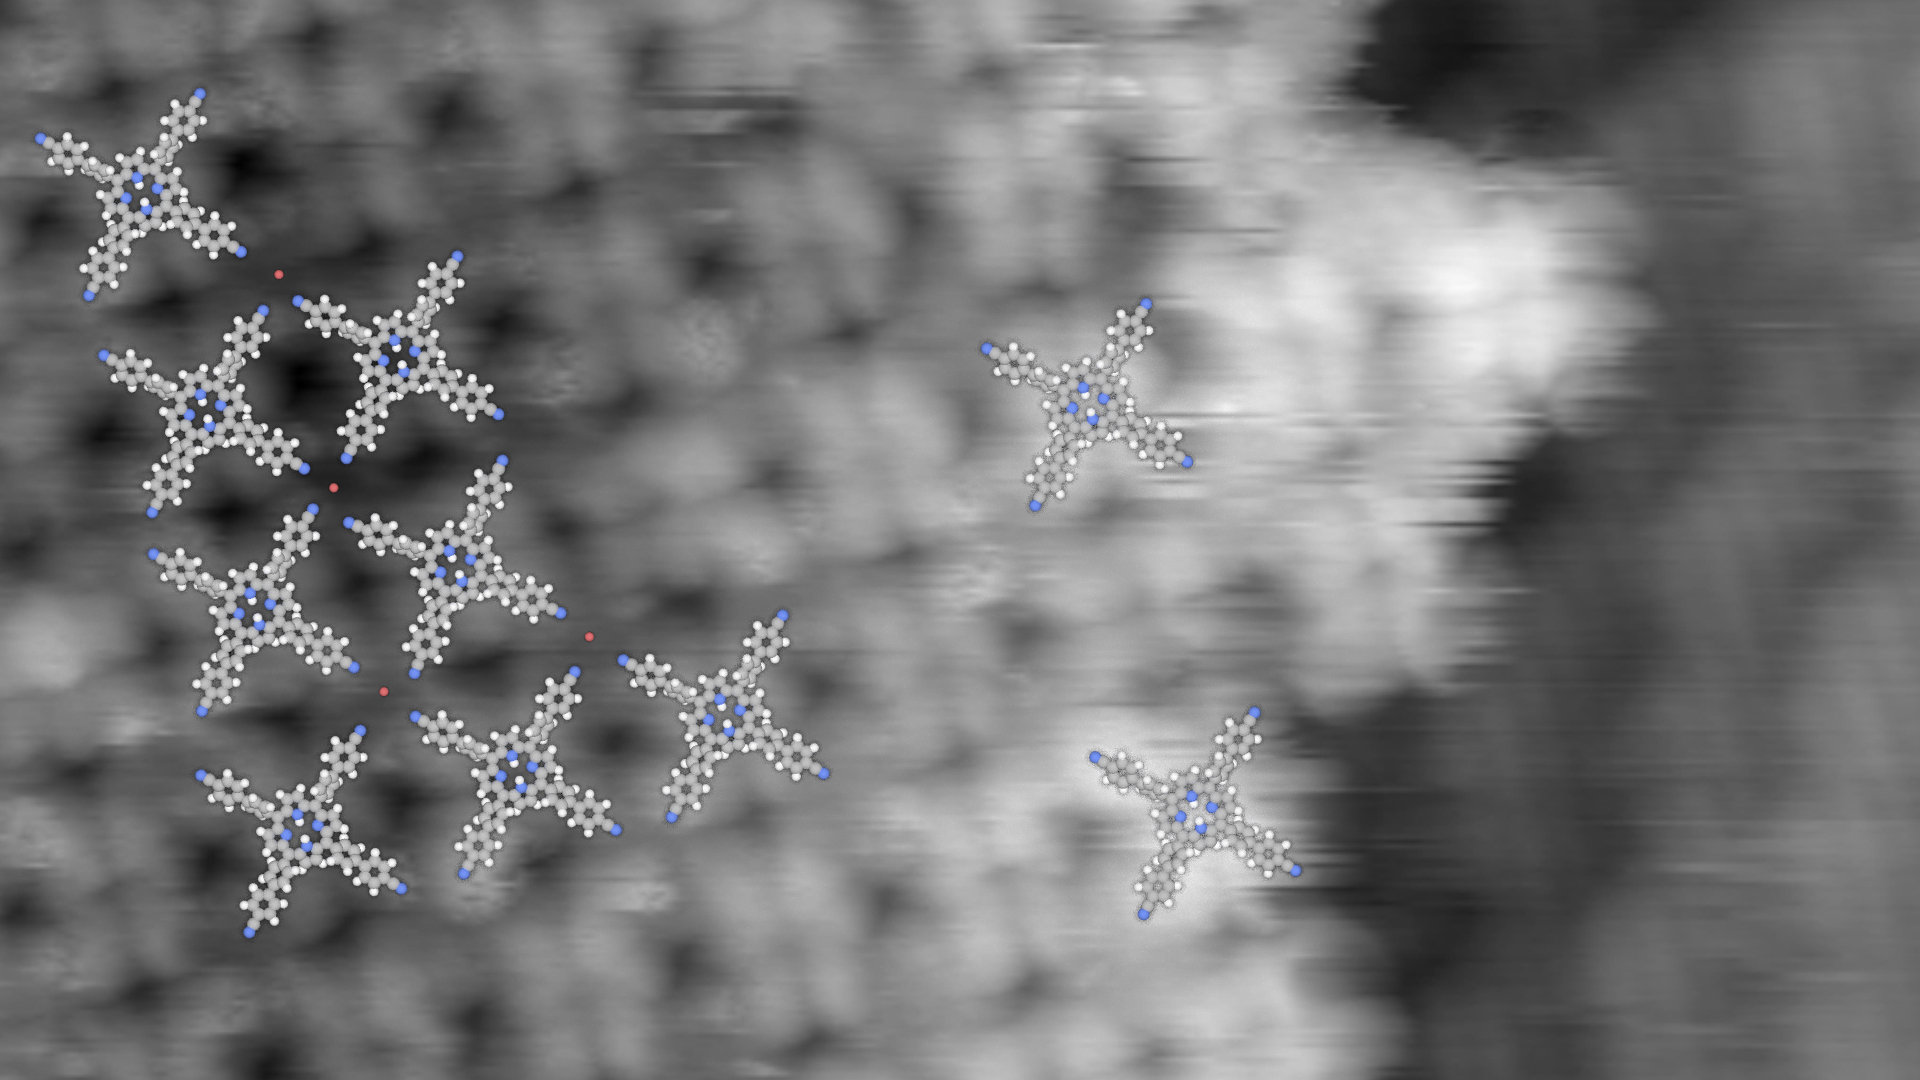
\includegraphics[width=0.45\textwidth]{./images/F150814-115601-cut1-overlay}
  }
\caption{Self-Assembled monolayer for TPCN on h-BN/Cu-foil. The cobald atoms sit right in between the molecules and faciliate a regular, ordered arrangement of the TPCN.}
\end{figure}

No sign for metallation (brighter center of porphine core) or cobald adatoms (bright spots in between the molecules) is observed. Because this type of binding is already reported \cite{urgel_controlling_2015}, similar binding mechanisms are derived for this system.

Molecules arrange periodically with center-center distances of about \SI{2.3}{\nano \meter}. This leaves a little void space in between 4 TPCN molecule's legs, space where a Co atom may be located. This would result in a distance of \SI{1.5}{\angstrom} between the end of a TPCN leg (its N-center) and the center of the cobald atom. Typical binding distances for Co-NC are reported \cite{schlickum_metalorganic_2007, przychodzen_supramolecular_2006} and in good agreement.

%---------- Build models in blender for correct spacings etc. ---------